\documentclass[conference]{IEEEtran}
\IEEEoverridecommandlockouts
\usepackage{amsmath,amssymb,amsfonts}
\usepackage{algorithmic}
\usepackage{graphicx}
\usepackage{textcomp}
\usepackage{xcolor}
\usepackage{tabularx}
\usepackage{geometry}
\geometry{
 a4paper,
 total={170mm,257mm},
 left=14.32mm,
 right=14.32mm,
 top=19mm,
 bottom=38mm,
}
\usepackage{balance}

\renewcommand\IEEEkeywordsname{Palabras clave}
\renewcommand{\refname}{Referencias}
\renewcommand\tablename{TABLA}

\begin{document}

\title{Codificación de audio filtrado digitalmente para implante coclear didáctico}

\author{
\IEEEauthorblockN{1\textsuperscript{st} Fabrizio Carlassara}
\IEEEauthorblockA{\textit{Laboratorio Sistemas embebidos} \\
\textit{UTN FRA}\\
Avellaneda, Argentina \\
fcarlassara@fra.utn.edu.ar}
\and
\IEEEauthorblockN{2\textsuperscript{nd} Pablo Gómez}
\IEEEauthorblockA{\textit{Laboratorio Tecnología Biomédica} \\
\textit{UTN FRA}\\
Avellaneda, Argentina \\
pablosgomez50@gmail.com}
\and
\IEEEauthorblockN{3\textsuperscript{rd} Ariel Marín}
\IEEEauthorblockA{\textit{Laboratorio Sistemas embebidos} \\
\textit{UTN FRA}\\
Avellaneda, Argentina \\
amarin@fra.utn.edu.ar}
\and
\IEEEauthorblockN{4\textsuperscript{th} Martín Enríquez}
\IEEEauthorblockA{\textit{Laboratorio Tecnología Biomédica} \\
\textit{UTN FRA}\\
Avellaneda, Argentina \\
martin.hernan.enriquez@gmail.com}
\and
\IEEEauthorblockN{5\textsuperscript{th} Ian Lesnianski}
\IEEEauthorblockA{\textit{Laboratorio Tecnología Biomédica} \\
\textit{UTN FRA}\\
Avellaneda, Argentina \\
ianlesni@gmail.com}
}

\maketitle

\begin{abstract}
Este trabajo presenta el desarrollo e implementación de un sistema de tramas de comunicación inalámbricas para estimulación multicanal, como parte de un implante coclear didáctico actualmente en desarrollo. El objetivo principal es diseñar una herramienta de bajo costo y consumo optimizado, orientada a su uso en contextos educativos. El sistema está basado en un microcontrolador Raspberry Pi Pico, elegido por su bajo consumo energético y facilidad de programación. Las tramas de datos se codifican mediante modulación por ancho de pulso (PWM) y se transmiten utilizando modulación por desplazamiento de amplitud (ASK) a través de una antena plana. Se diseñaron tramas diferenciadas para configurar el modo de estimulación y establecer los parámetros de cada canal. Las pruebas preliminares demostraron la viabilidad de la transmisión y decodificación de las tramas mediante acoplamiento inductivo.
\end{abstract}

\begin{IEEEkeywords}
\textit{implante coclear, modulación ASK, Raspberry Pi Pico, PWM, comunicación inalámbrica}
\end{IEEEkeywords}

\section{Introducción}

La pérdida auditiva profunda bilateral afecta de forma significativa la calidad de vida de quienes la padecen, limitando su capacidad de comunicación e interacción social. En este contexto, los implantes cocleares han demostrado ser una solución eficaz, proporcionando una vía alternativa de percepción sonora mediante estimulación eléctrica directa del nervio auditivo \cite{eshraghi2012_history_future} . Sin embargo, el alto costo, la complejidad tecnológica y los requerimientos quirúrgicos limitan su acceso en países en desarrollo y dificultan su comprensión por parte de estudiantes e investigadores que se inician en la ingeniería biomédica y la audiología \cite {ramos2016_implante_estado} 

\begin{figure}[h!]
\centering
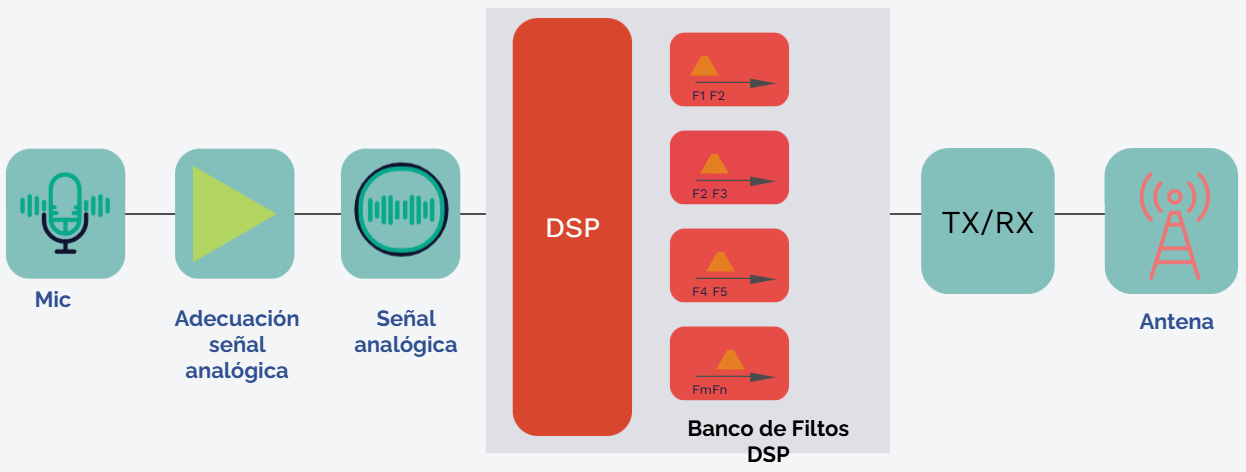
\includegraphics[width=0.5\textwidth]{assets/block_diagram_external_unit.png}
\caption{Bloques funcionales del módulo externo del sistema. La señal acústica captada por el micrófono se acondiciona y procesa digitalmente mediante un banco de filtros realizados con Digital Signal Processor (DSP). La información codificada se transmite de forma inalámbrica al módulo interno a través de una antena.}
\label{fig:block_diagram_external_unit}
\end{figure}

El presente trabajo se enmarca en un proyecto de investigación y desarrollo orientado al diseño de un implante coclear con fines didácticos \cite{nidcd2016_implantes},  cuyo objetivo principal es facilitar la enseñanza de los principios fundamentales de los sistemas implantables, el procesamiento de señales biomédicas y la bioelectrónica.

Los bloques funcionales del sistema pueden dividirse en dos módulos principales: uno externo y otro implantado. La Fig. \ref{fig:block_diagram_external_unit} muestra el diagrama funcional del módulo externo, donde la señal acústica captada por el micrófono es acondicionada y procesada digitalmente para luego ser codificada y transmitida por una antena plana. El módulo interno tiene como objetivo recibir, decodificar y luego estimular apropiadamente el electrodo correspondiente al estímulo solicitado.

Particularmente, este artículo se enfoca en el módulo externo, buscando filtrar digitalmente una señal de audio, caracterizarla y luego codificarla y transmitirla. Se buscó obtener resultados preliminares de la viabilidad tecnológica de un dispositivo de estas características.

\section{Marco teórico - fundamentos}

Para poder transmitir a través del acople inductivo los datos procesados por el Digital Signal Procesing (DSP) al dispositivo implantado fue necesario definir algunos criterios que se describirán en las secciones siguientes:

\begin{enumerate}
    \item Implementación de filtros y características.
    \item Codificación de la información.
    \item Estrategia de transmisión y recepción.
\end{enumerate}

\subsection{Implementación de filtros y características}

Lo primero a definir resulta ser la banda de frecuencias útiles y la cantidad de electrodos a estimular. En esta implementación, se decidió buscar un rango útil de frecuencias hasta 4 kHz con un total de 8 electrodos. Esto resulta en ocho bandas de frecuencias como se ve en la Tabla \ref{table:freq_bands}.

\begin{table}[h!]
\centering
\caption{Banda de frecuencias asignadas a cada canal de estimulación.}
\label{table:freq_bands}
\begin{tabularx}{\columnwidth}{|c|X|X|X|}
    \hline
    \multicolumn{4}{|c|}{Banda de frecuencias asignadas a cada canal de estimulación} \\
    \hline
    Banda & Corte Inferior (Hz) & Central (Hz) & Corte Superior (Hz) \\
    \hline
    1 & 365.2 & 424.1 & 492.6 \\
    2 & 492.6 & 572.1 & 664.4 \\
    3 & 664.4 & 771.6 & 896.1 \\
    4 & 896.1 & 1040.7 & 1208.6 \\
    5 & 1208.6 & 1403.7 & 1630.2 \\
    6 & 1630.2 & 1893.2 & 2198.8 \\
    7 & 2198.8 & 2553.6 & 2965.6 \\
    8 & 2965.6 & 3444.2 & 4000.0 \\
    \hline
\end{tabularx}
\end{table}

Una vez definido el rango de frecuencias, se optó por usar un filtrado digital con FFT, teniendo que definir la cantidad de muestras y la frecuencia de muestreo necesaria, encontrando un equilibrio entre el tiempo dedicado a muestrear la señal y la resolución obtenida.

Se decidió trabajar a una frecuencia de muestreo de 16 kHz, lo que cumple el criterio de muestreo de Nyquist y tener un total de 512 muestras, lo que garantiza un error de 31.25 Hz en el resultado de la FFT con un tiempo de adquisición de alrededor 32 ms. 

\begin{table}
\centering
\caption{Mapeo de bandas a canales de estimulación.}
\label{table:freq_bins}
\begin{tabularx}{\columnwidth}{|c|X|X|X|}
    \hline
    \multicolumn{4}{|c|}{Mapeo de bandas a canales de estimulación} \\
    \hline
    Banda & Indice de corte inferior & Indice de corte superior & Cantidad de muestras \\
    \hline
    1 & 11 & 15 & 5 \\
    2 & 16 & 21 & 6 \\
    3 & 22 & 28 & 7 \\
    4 & 29 & 38 & 10 \\
    5 & 39 & 52 & 14 \\
    6 & 53 & 70 & 18 \\
    7 & 71 & 94 & 24 \\
    8 & 95 & 128 & 34 \\
    \hline
\end{tabularx}
\end{table}

Finalmente, los valores resultantes de la FFT se agrupan en 8 bandas de frecuencias donde se obtendrá el promedio de energía para luego poder mandar al estimulador. En la Tabla \ref{table:freq_bins} se puede ver la cantidad de valores de salida de la FFT que corresponden a cada banda.

\subsection{Codificación de la información}

El sistema de estimulación se basa en la transmisión secuencial de tramas codificadas que definen el modo de operación y los parámetros de estimulación eléctrica. Se diseñaron dos tipos de tramas diferenciadas que denominaremos \textbf{Trama A}, destinada a configurar el modo de estimulación y la duración de los pulsos, y la \textbf{Trama B} utilizada para establecer el canal (electrodo) y la amplitud de estimulación. La combinación de ambas permite definir secuencias con flexibilidad, manteniendo la simplicidad de decodificación y la robustez del protocolo.

Para los propósitos de este artículo, sólo la Trama B fue implementada tal como se puede ver en la Fig. \ref{fig:implant_data}.

\begin{figure}[h!]
\centering
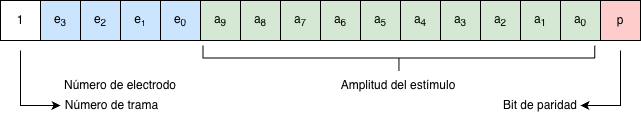
\includegraphics[width=0.48\textwidth]{assets/implant_data.png}
\caption{Trama de datos para la configuración del electrodo de estimulación y la amplitud del pulso (Trama B).}
\label{fig:implant_data}
\end{figure}

Como se puede ver, la trama está compuesta por dieciséis bits de datos, agrupados de la siguiente forma:

\begin{itemize}
    \item Bit 15: siempre en 1 para esta trama y para cualquier electrodo ya que corresponde a la Trama B.
    \item Bits 14-11: número de electrodo. Teniendo cuatro bits disponibles, esta trama permitiría diferenciar hasta dieciséis electrodos distintos.
    \item Bits 10-1: amplitud del estímulo. Con diez bits de resolución, es posible obtener una buena precisión en la estimulación de cada electrodo asignado a cada banda.
    \item Bit 0: bit de paridad para chequear errores.
\end{itemize}

\subsection{Estrategia de transmisión y recepción}

Para enviar la información codificada, se eligió un tipo de transmisión por PWM a 2 MHz, frecuencia a la que está sintonizada la antena plana que se usará para transmitir la información al módulo interno.

La estrategia que se usó para diferenciar los distintos datos en la trama es la siguiente y puede verse en la Fig. \ref{fig:implant_codification}:

\begin{itemize}
    \item Un cero lógico es representado por seis pulsos consecutivos de 50\% de ancho de pulso, seguido por diez pulsos de 0\% de ancho de pulso.
    \item Un estado idle o sin datos se representa con nueve pulsos consecutivos de 50\% de ancho de pulso, seguido por siete pulsos de 0\% de ancho de pulso.
    \item Un uno lógico es representado por doce pulsos consecutivos de 50\% de ancho de pulso, seguido por cuatro pulsos de 0\% de ancho de pulso.
\end{itemize}

\begin{figure}[h!]
\centering

\includegraphics[width=0.48\textwidth]{assets/implant_codification.png}
\caption{Esquema de codificación de bits utilizando modulación por ancho de pulso (PWM). Se representa el ciclo de trabajo correspondiente al bit lógico “0” (seis pulsos), al bit “idle” (nueve pulsos) y al bit lógico "1" (doce pulsos).}
\label{fig:implant_codification}
\end{figure}

Este tipo de estrategia para modular la información como ASK fue elegida por su simplicidad, bajo consumo y facilidad de implementación en microcontroladores y se evita la complejidad de métodos como FSK o PSK. ASK resulta especialmente adecuada para enlaces inductivos por su eficiencia y robustez ante desplazamientos de fase \cite{zierhofer1996_geomagnetic_coils}. 

La frecuencia de los pulsos es de 2 MHz para poder transmitir con facilidad los datos a través de la antena, sin embargo, se eligió codificar los bits como una secuencia de pulsos de ancho de pulso fijo y no variable. Un bit de datos en esta codificación corresponde a un total de dieciséis ciclos de 2 MHz, dando un tiempo total de 8 $\mu$s. La razón de armar secuencias de pulsos de seis, nueve y doce pulsos completando los dieciséis ciclos con la linea en cero es porque esto representa un 40\%, 60\% y 80\% de ancho de pulso de una señal de 125 kHz.

\begin{figure}[h!]
\centering

\includegraphics[width=0.25\textwidth]{assets/implante_decodificacion.png}
\caption{Ciclos de trabajo del lado del receptor. Se representa el ciclo de trabajo correspondiente al bit lógico "0" (40\%), al bit "idle" (60\%) y al bit lógico "1" (80\%)}
\label{fig:implant_decodification}
\end{figure}

Esta nueva codificación de pulsos es posible ya que desde el lado del receptor, se prevee usar un detector de envolvente que termina inyectando al microcontrolador de la unidad interior señales como las que se ven en la Fig. \ref{fig:implant_decodification}. Al ser señales de mucha más baja frecuencia, es posible recibir y decodificar con mucha más facilidad en el microcontrolador del receptor, usando los anchos de pulsos variables como referencia para diferenciar un estado de otro.

\section{Metodología e implementación}

La implementación de toda la adquisición, procesamiento, transmisión y generación de tramas de datos fue hecha sobre una Raspberry Pi Pico 2, una pequeña placa de desarrollo con un RP2350 \cite{raspberrypi2024_rp2350_datasheet} de Raspberry Pi con un doble Córtex-M33. Algunas características de este mirocontrolador que son beneficiosas para esta implementación incluyen:

\begin{itemize}
    \item El Cortex-M33 tiene unidad de punto flotante (FPU) lo que facilita trabajar con valores flotantes con mayor precisión y velocidad, útil especialmente para el procesamiento de señales.
    \item Tiene dos núcleos Cortex-M33, lo que permitiría repartir tareas en ambos procesadores para que la implementación sea más eficiente.
    \item El procesador tiene un clock de 150 MHz, lo que nos ayudará a poder procesar datos y generar tramas con mucha velocidad.
    \item Tiene 512 kB de memoria RAM, más que suficiente para almacenar una buena cantidad de muestras.
    \item ADC de 12 bits a 500 kS/s que nos alcanza para muestrear audio con suficiente resolución.
    \item PWM y PIO (Programmable Input Output) que nos servirá para generar las tramas de datos.
\end{itemize}

\subsection{Adquisición y procesamiento digital}

La señal captada por el módulo ADC (Analog to Digital Converter) interno del RP2350 a una frecuencia muestreo de 16 kHz configurando apropiadamente el clock del conversor. Estos datos se almacenan en buffers de forma secuencial por medio de interrupciones del módulo DMA (Direct Access Memory), los buffers se gestionan de forma cíclica para obtener un flujo continuo de datos sin riesgo a que se corrompan los datos que se procesan debido a un nuevo muestreo en proceso.

Para el procesamiento de señales mediante una FFT, se recurrió a una biblioteca estandarizada y optimizada para Cortex-M33 llamada CMSIS DSP que aprovecha las características de estos procesadores como lo son la FPU. Esta ya cuenta con funciones que aplican una FFT a un buffer de datos, permitiendo agilizar mucho el tiempo de procesamiento de la señal.

Una vez procesados los datos, se aplican filtros según las frecuencias planteadas en la Tabla \ref{table:freq_bins} y se procede a obtener el promedio de energía de cada banda para proceder a codificar.

\subsection{Generación de tramas desde el transmisor}

La primer estrategia implementada fue usar el propio PWM y Timer del RP2350. La idea sería lograr que ciclo a ciclo se actualice el ancho de pulso a 50\% o 0\% de acuerdo al número de ciclo que se esté generando del bit de datos deseado.

Sin embargo, para garantizar que los tiempos son los especificados para la transmisión, es necesario usar interrupciones y, generándolas cada ciclo que se quiera enviar implicaría que cada 500 ns se estarían disparando interrupciones. Debido al tiempo que toma resolver cada interrupción y lo que el programa principal debe hacer a la vez, se concluyó que no era una buena estrategia dados los requisitos del sistema.

Como alternativa, se decidió usar el PIO del RP2350. Este consiste en una máquina de estado dedicada que puede asociarse a un GPIO y programarse con un set de instrucciones propio, corriendo independientemente del procesador.

El PIO del RP2350 cuenta con registros propios (X e Y) que comparte con el procesador y es capaz de generar interrupciones. Estos recursos van a permitir que se delegue la confección de las tramas de datos en el PIO sin sobrecargar al procesador de interrupciones que atender.

\begin{figure}
\centering
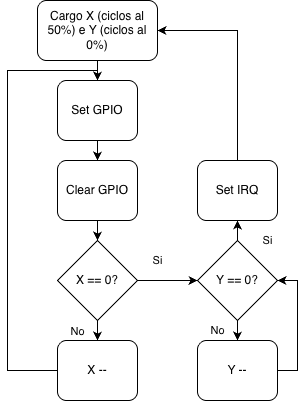
\includegraphics[width=0.4\textwidth]{assets/pio_flow_chart.png}
\caption{Diagrama de flujo del generador de tramas implementado en el PIO.}
\label{fig:pio_flow_chart}
\end{figure}

En la Fig. \ref{fig:pio_flow_chart} se puede ver la lógica implementada en la máquina de estados. La implementación es sencilla, simplemente el procesador carga los registros compartidos con la cantidad de ciclos que tiene que generar el PIO con el 50\% de ciclo de trabajo y cuántos con 0\% y luego de generarlos todos, interrumpe al procesador, permitiendo que las interrupciones sean cada 8 $\mu$s, lo que es mucho más manejable.

En cuanto a la garantía que existe de que los tiempos del PIO sean los requeridos, cada instrucción que ejecute éste se resuelve en un ciclo de clock del PIO, por lo que es posible asignar un clock conocido y determinar con precisión lo que demora el PIO en resolver cada instrucción para generar toda la trama.

\section{Ensayos}

Para ensayar, se inyectó al ADC una señal conocida y se evaluó con un analizador lógico la salida que iría al módulo interno.

En la Fig. \ref{fig:test_full} se toma como referencia la 2da trama que se envió. Se puede ver que la trama efectivamente queda conformada por 16 bits de datos con 125 $\mu$s de período, garantizando la frecuencia de 125 kHz que se buscaba para el receptor.

En la trama se ve el dato 0x8900, indicando que es el segundo estímulo enviado con una amplitud de 128 ya que la señal testeada tenía mayor concentración de energía en la segunda banda.

\begin{figure}
\centering
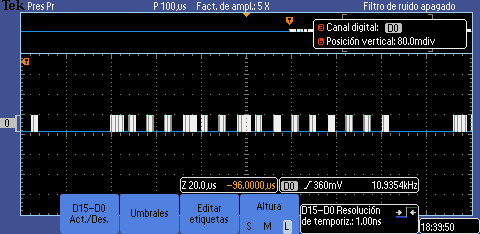
\includegraphics[width=0.48\textwidth]{assets/TEK00003.PNG}
\caption{Vista completa de la 2da Trama B}
\label{fig:test_full}
\end{figure}

En la Fig. \ref{fig:test_zoom} se puede ver el comienzo de la quinta trama de datos, donde se puede ver más en detalle la conformación de pulsos. Se puede corroborar que los bits lógicos altos son conformados por doce pulsos consecutivos de 2 MHz mientras que los bits lógicos bajos se conforman por seis pulsos consecutivos.

\begin{figure}
\centering
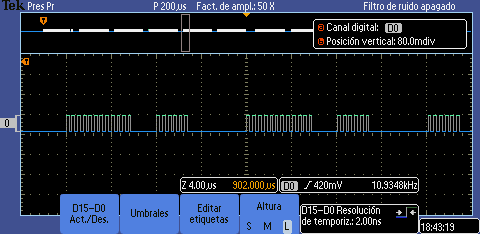
\includegraphics[width=0.48\textwidth]{assets/TEK00011.PNG}
\caption{Comienzo de la 5ta Trama B generada}
\label{fig:test_zoom}
\end{figure}

\section{Conclusiones}

Los ensayos preliminares mostraron que el flujo de datos desde la adquisición de la señal hasta la generación de la trama de datos es lograble bajo los estándares impuestos para el prototipo didáctico propuesto.

Además, fue fundamental la selección de un microcontrolador como el RP2350, con características que facilitan mucho el procesamiento de datos. El acceso a una FPU, la gran velocidad de clock y el uso de bibliotecas optimizadas permitió que el uso de algoritmos de procesamiento como el de FFT sean más viables y rápidos y al mismo tiempo permitirnos el beneficio de tener respuestas de filtros de banda muy precisos.

Queda pendiente trabajar en la selección de la cantidad de muestras, la resolución que se desea obtener y la frecuencia de muestreo. Esta combinación de parámetros elegidos, si bien cumplen con las especificaciones planteadas, limitan la velocidad a la que se termina transmitiendo la trama de datos debido al tiempo en el que se tarda en tomar todas las muestras. Esto presenta un posible problema ya que podría introducir mucha latencia en el módulo interno y finalmente en la escucha del usuario. Queda evaluar un uso más eficiente de estrategias de muestreo o incluso de filtrado, quizás evaluando distintos tipos de filtro frente a los implementados con FFT.

\bibliographystyle{IEEEtran}
\bibliography{references}
\nocite{*}
\balance

\end{document}
